% !TEX program = lualatex
\documentclass[../../main.tex]{subfiles}
\begin{document}

\subsubsection{Representation}

For breadth first search the representation is a tree where each node can have 0-4 children because of the branch factor.

\subsubsection{Characteristics of breadth first search}

Breadth first mostly makes sense when the distance between nodes are equal and
will find the shortest path if it exists.

This breadth first solution generates a new state for each player step.

The worst case states generated can be calculated as:

\begin{equation}
	\textrm{empty squares}^{ \textrm{Number of boxes}}
\end{equation}

This infers that the number of boxes is the determining factor for the size
of the generated tree from breadth first search.

The worst case time complexity can be calculated as

\begin{equation}
	4^{  \left(  \textrm{Empty Squares} ^{ \textrm{Number of Boxes}}  \right)   }
\end{equation}

This will probably always be lower as it is not always possible to move in all 4 direction.

This makes it possible to generate a path by walking up the tree all the way up to the root after the correct state have 	been found.

A small comparison of deadlock detection disabled and enabled shows that without detection, breadth first search generates 1306496 nodes while consuming a bit over 2 GB of ram. The time to find the solution is about 59 seconds depending on the computer that is used.
With deadlock detection 206932 nodes are created with about 1 GB of ram. Time to find a solution was decreased to about 9.5 seconds.

\subsubsection{Solver results}

This section shows the Breadth First Search results of the levels that was handed out during the course.

\paragraph{First level}

\begin{figure}[h]
	\centering
	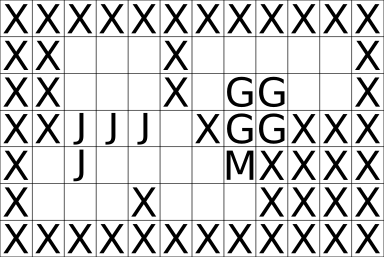
\includegraphics[width=0.4\linewidth]{images/level_1.png}
	\label{fig:images/level_1}
	\caption{Level 1}
	\label{fig:level_1}
\end{figure}

 \begin{itemize}

	\item Runtime 		
 		
 	BFS has a runtime of about 9.5 seconds
 		
	\item Memory usage
		
	BFS has a memory consumption of about 1 GB on the first level
	
	\item Amount of nodes created
	
	BFS creates 206932 nodes
	
	\item Solution step length
	
	BFS generates a solution that has 108 steps
	
	\item Solution string
	
	lllldlluRRUdRRRdrUUruulldRRdldlluLuulldRurDDullDRdRRRdrUUruurrdLulDulldRddlllldlluRRRRRdrUUdlllluurDldRRRdrU
		
 \end{itemize}

\paragraph{Second level}

\begin{figure}[h]
	\centering
	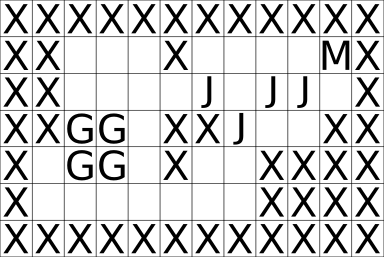
\includegraphics[width=0.4\linewidth]{images/level_2.png}
	\label{fig:images/level_2}
	\caption{Level 2}
	\label{fig:level_2}
\end{figure}

\begin{itemize}

	\item Runtime 		
 		
 	BFS has a runtime of about 14 seconds
 		
	\item Memory usage
		
	BFS has a memory consumption of about 1.3 GB on the second level
	
	\item Amount of nodes created
	
	BFS creates 357829 nodes
	
	\item Solution step length
	
	BFS generates a solution that has 83 steps
	
	\item Solution string
	
	llDlLLLLrrrrrurrdLLLLLLulDDrddrrruUddllluLruurrurrrddLuLLLLulDDrddrrruUruLLLLulDulD
		
 \end{itemize}

\end{document}
